\documentclass[border=10pt]{standalone}
\usepackage{tikz}
\usetikzlibrary{arrows.meta, shapes, calc}

\begin{document}
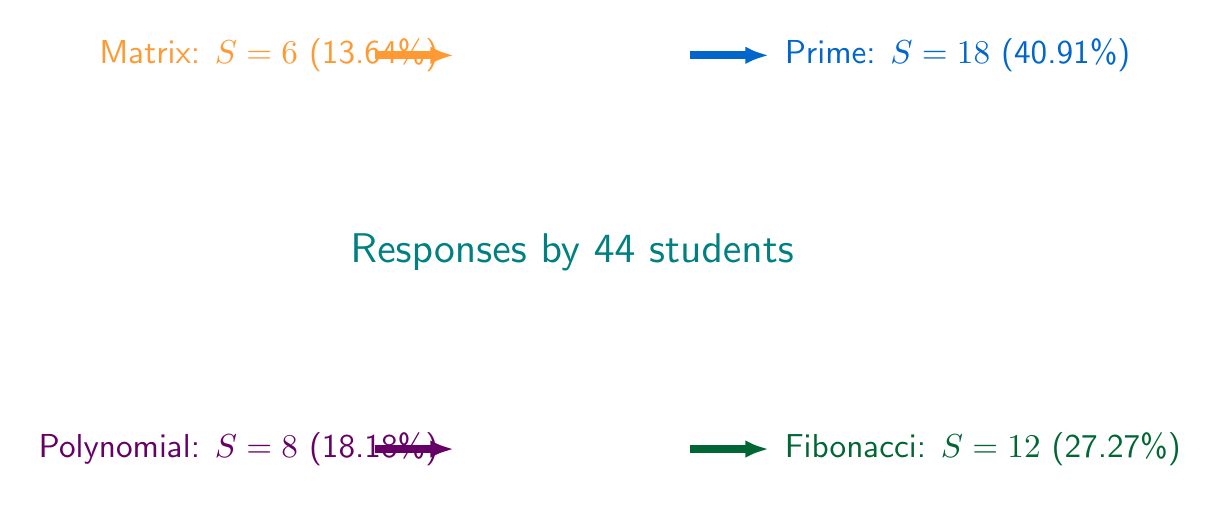
\begin{tikzpicture}[font=\sffamily]

% Define colors
\definecolor{color1}{RGB}{0, 102, 204}
\definecolor{color2}{RGB}{255, 153, 51}
\definecolor{color3}{RGB}{102, 0, 102}
\definecolor{color4}{RGB}{0, 102, 51}

% Donut chart segments
\newcommand{\donutchart}[1]{
    \pgfmathsetmacro{\totalnum}{0}
    \foreach \value/\colour/\name in {#1} {
        \pgfmathparse{\value+\totalnum}
        \global\let\totalnum=\pgfmathresult
    }

    \begin{scope}[rotate=90]

    \pgfmathsetmacro{\wheelwidth}{0.3}
    \pgfmathsetmacro{\midradius}{1+\wheelwidth/2}

    \foreach \value/\colour/\name in {#1} {
        \pgfmathsetmacro{\angle}{360*\value/\totalnum}
        \pgfmathsetmacro{\midangle}{(\pgfmathresult/2)+\pgfmathresult}

        \fill[\colour] (0,0) -- (\midangle:\midradius pt+\wheelwidth/2) arc (\midangle:\midangle+\angle:\midradius pt+\wheelwidth/2) -- cycle;
        \draw[white, line width=0.3cm] (0,0) -- (\midangle:\midradius pt+\wheelwidth/2) arc (\midangle:\midangle+\angle:\midradius pt+\wheelwidth/2) -- cycle;

        \pgfmathsetmacro{\temp}{\midangle+\angle/2}
        \node[scale=0.8, text=white] at (\temp:\midradius pt) {\name};

        \global\let\cumnum=\pgfmathresult
    }

    \end{scope}
}

% Data for the donut chart
\donutchart{18/color1/Prime, 6/color2/Matrix, 8/color3/Polynomial, 12/color4/Fibonacci}

% Central text
\node[scale=1.5, text=teal] at (0,0) {Responses by 44 students};

% Labels and arrows
\draw[-{Latex[length=3mm]}, color1, line width=1mm] (1.5, 2.5) -- (2.5, 2.5) node[right, scale=1.2, color1] {Prime: $S=18$ (40.91\%)};
\draw[-{Latex[length=3mm]}, color2, line width=1mm] (-2.5, 2.5) -- (-1.5, 2.5) node[left, scale=1.2, color2] {Matrix: $S=6$ (13.64\%)};
\draw[-{Latex[length=3mm]}, color3, line width=1mm] (-2.5, -2.5) -- (-1.5, -2.5) node[left, scale=1.2, color3] {Polynomial: $S=8$ (18.18\%)};
\draw[-{Latex[length=3mm]}, color4, line width=1mm] (1.5, -2.5) -- (2.5, -2.5) node[right, scale=1.2, color4] {Fibonacci: $S=12$ (27.27\%)};

\end{tikzpicture}
\end{document}